\documentclass[review]{elsarticle}
\usepackage{hyperref}
\usepackage[margin=1in]{geometry}
\usepackage{graphicx}
\usepackage{amsmath}
\usepackage{placeins}
\usepackage{comment}
\usepackage{gensymb}


\journal{Journal of Nuclear Materials}
\bibliographystyle{elsarticle-num}

\begin{document}
\begin{frontmatter}
\title{Calculation of the displacement energy of $\alpha$ and $\gamma$ uranium}

\author[inl]{Benjamin Beeler\corref{qwe}}
\cortext[qwe]{Corresponding author}
\ead{benjamin.beeler@inl.gov}
\author[inl]{Yongfeng Zhang}
\author[pur]{Maria Okuniewski}
\author[gatech]{Chaitanya Deo}
\address[inl]{Idaho National Laboratory, Idaho Falls, ID 83415}
\address[pur]{Purdue University, West Lafayette, IN 47907}
\address[gatech]{Georgia Institute of Technology, Atlanta, GA 30332}

\begin{abstract}

Uranium is alloyed with Mo or Zr in order to stabilize the high-temperature body-centered cubic $\gamma$ phase of uranium for use in nuclear reactors. Although these two alloy systems possess different mechanical, chemical and thermodynamic properties, they exhibit a similarity in that there exists a variable degree of phase decomposition from the cubic $\gamma$ phase of uranium to the orthorhombic $\alpha$ phase of uranium, depending on both the Mo/Zr content and fabrication conditions. These two phases of uranium are believed to exhibit distinct swelling and radiation damage behavior. Understanding the differences in behavior under irradiation between the $\alpha$ and $\gamma$ phases can provide valuable information to guide the manufacturing process of U alloys and can inform multi-physics, continuum-level fuel performance codes. The threshold displacement energy (TDE) is the minimum amount of kinetic energy required to displace an atom from its lattice site. It is critically important to determine an accurate value of the TDE in order to calculate the total number of displacements due to a given irradiation condition, and thus to understand the materials response to irradiation. In this study, molecular dynamics simulations have been performed to calculate the displacement energy for both the $\alpha$ and $\gamma$ phases of uranium as a function of temperature. This study utilizes three different interatomic potentials that have been previously developed: U MEAM, UZr MEAM and UMo ADP. The displacement energy in $\gamma$U at 800 K is 74.5 eV, 47.0 eV and 35.6 eV for the U MEAM, UZr MEAM and UMo ADP potentials. respectively. The displacement energy for $\alpha$U at 600 K is 66.2 eV for the UMo ADP. 
\end{abstract}
\end{frontmatter}

\section{Introduction}

In the interest of nuclear non-proliferation, there has been renewed interest in recent decades to replace current highly enriched uranium (HEU) fuel in high power research reactors with low enriched uranium (LEU) fuel \cite{snelgrove1997}. In the United States, this program is the United States High-Performance Research Reactor (USHPRR) program. Research reactors require fuel that operates at high power and reaches high fission density, but at relatively low temperatures. Typical research reactor fuel consists of aluminum (Al) cladding surrounding a fuel meat composed of fuel particles dispersed in an Al matrix \cite{meyer2014}. In order to achieve a reduced enrichment in these fuel types, there is a requirement for increased uranium density. One way this is achieved is by utilizing $\gamma$ stabilized uranium alloys with 10 wt.\% or less alloy content. The fuel design being pursued under the USHPRR program is a uranium-molybdenum (U-Mo) monolithic foil, with a zirconium (Zr) diffusion barrier in Al clad. 

Uranium-zirconium (U-Zr) and uranium-plutonium-zirconium (U-Pu-Zr) alloy fuels have a history of usage in sodium-cooled fast reactors. Not only does the U-Zr fuel (as well as U-Pu-Zr) generate a harder neutron spectrum as compared to traditional ceramic fuels, but it also offers excellent neutron economy and high burnup capability \cite{hofman1997}. Recently, U-Zr fuels have regained interest due to the possibility of incorporating minor actinides into the fuel, and as such the metallic fuel alloys would serve to reduce the quantity of long-lived radioisotopes present in nuclear waste \cite{capriotti2017}. 

One issue with metallic fuels, including both UZr and UMo fuels, is the large amount of swelling that takes place \cite{hofman1997}. Such swelling can be accounted for in the fuel design, however the swelling needs to be stable and predictable up to high fission densities. Research reactor fuel types based on UMo are unique in that there cannot exist fission gas release from the fuel, and as such there is a relatively high content of fission gas and of fission gas bubbles within the fuel matrix. This importance of swelling in addition to the unique fuel environment has led to a variety of studies attempting to characterize the swelling behavior in U-Mo fuels \cite{rest2009, kim_anl08, meyer2002, kim2013} which has led to the development of a swelling correlation from Argonne National Labortory (ANL correlation) \cite{kim2011} as a function of fission density. This swelling correlation was intended to be applicable for low temperature (less than 250$^{\circ}$C) U-Mo alloys in the 7-10 wt.\% composition range. 

A 2015 post-irradiation examination (PIE) report \cite{afip6report} showed early onset break-away swelling in U-10Mo fuels at fission densities much lower than previously observed. This fuel swelling behavior deviated from the ANL correlation and such behavior could lead to early fuel failure. Understanding the cause of this anomalous swelling behavior is a critical step in qualifying U-Mo fuel for use in research reactors. This PIE report showed a large amount of compositional banding, or regions of low Mo content adjacent to regions of higher Mo content, in the as-fabricated fuel. An increased amount of swelling was also observed in lower Mo content alloys (U-7Mo) \cite{vandenberghe2014} at lower fission densities. Lower Mo content leads to phase transformation from the $\gamma$U-Mo body-centered cubic phase to the $\alpha$U phase and U$_{2}$Mo \cite{janfong2014}. This is most evident in the region involving the U-Mo fuel foil and the Zr diffusion barrier \cite{park2015}. Near the Zr diffusion barrier, there exists a limited region of interaction where there exists a variety of phases including $\gamma$U-Mo, UZr$_{2}$, Mo$_{2}$Zr and $\alpha$U. This inter-diffusion region exhibits the highest density of fission gas bubbles at high fission densities and is the region where fuel separation initiates \cite{rertr12}. Finally, an earlier onset of recrystallization has been observed in alloys with either lower Mo content or increased banding \cite{kim2013A}. Recrystallization is the suggested culprit behind break-away swelling, as the recrystallized grains are destroying the fission gas superlattice \cite{vandenberghe2008}. 

U-Zr alloys are typically employed as a series of fuel pellets within a given fuel rod, similar to UO$_{2}$ fuels. Unlike UO$_{2}$ fuels, dramatic swelling is inevitable, and is typically accounted for by manufacturing fuels with a smear density of approximately 75{\%}. This allows for approximately 30\% swelling, which is sufficient to allow fission gas release \cite{beck1968}. The nature of swelling is anisotropic in these fuels, largely due to the difference in swelling behavior between the hotter center of the fuel and the colder periphery \cite{hofman1990}. The degree of anisotropicity increases with increasing Pu content. During operation, the phenomenon of constituent redistribution takes place. This results in three distinct radial phase regions within the fuel. The innermost region is Zr-rich, the intermediate region is Zr-poor and the outermost region has a nominal Zr concentration. This phenomenon is due to both the effect of the temperature gradient on phase equilibria and the diffusion of species along the temperature gradient. This concentration variance as a function of radius in combination with the temperature gradient leads to the $\gamma$ phase being present in the interior of the fuel pellet, while the $\alpha$ phase dominates the periphery \cite{kobayashi1990, kim2004}. The radially anisotropic swelling within the fuel pellet is due to the variation in phases as a function of radius.

This information suggests that there is a fundamental difference between the radiation damage behavior and swelling behavior of the $\alpha$ phase of U and the $\gamma$ phase of U (UMo/UZr). The first step to unraveling this puzzle is to investigate the radiation damage-related properties of both $\alpha$ U and $\gamma$ U.

One of the most fundamental quantities of radiation damage is the threshold displacement energy (TDE). The TDE is defined as the minimum amount of kinetic energy required to displace an atom from its lattice site. This quantity plays a key role in radiation damage theory, where it is implemented within the Kinchin-Pease \cite{kinchinpease} or the Norgett-Robinson-Torrens (NRT) \cite{norgett1975} equations, which state that the amount of damage is proportional to the ratio of the amount of deposited energy to an effective TDE. Therefore, it is critically important to determine an accurate value of the TDE in order to calculate the total number of displacements due to a given irradiation condition, and thus understand the materials response to irradiation.

In this paper, molecular dynamics (MD) simulations have been performed to calculate the TDE in $\alpha$ and $\gamma$U at 600 K, 800 K and 1000 K utilizing three unique interatomic potentials. The probability of Frenkel pair (vacancy and interstitial pair) production is determined as a function of PKA direction and temperature. Probability curves are averaged to determine an effective value of the TDE, above which a Frenkel pair is more than 50$\%$ likely to form. 

\section{Computational Details}
In order to determine the TDE at temperatures of interest for nuclear reactors, molecular dynamics (MD) \cite{abraham1986, allen1987} simulations need to be performed. MD requires an interatomic potential to describe the energy landscape of the system being studied. Very few interatomic potentials have been constructed for uranium-based alloys. This is due to the inherent difficulty in describing the behavior of f-electrons and the mechanical instability of the $\gamma$ phase of uranium at low temperatures. Several interatomic potentials have been developed for pure uranium \cite{beeler_meam, beelerASTM, fernandez2014, li2011, smirnova2012, li2012}, with only a few being adapted into alloy potentials for U-Zr \cite{moore2015}, U-Al \cite{pascuet2012}, U-Si \cite{beelerUSi} and U-Mo \cite{smirnovaUMo}. The modified embedded-atom method (MEAM) variants of U and U-Zr \cite{beeler_meam, moore2015} are the two potentials that can most accurately describe the $\gamma$ phase of uranium, and the pure U MEAM potential \cite{beeler_meam} has been utilized for a prior radiation damage study \cite{miao2015}. However, the pure U MEAM potential is incapable of accurately describing the $\alpha$ phase. The U-Zr variant of the MEAM potential is an updated version of the prior pure U MEAM potential that was modified to accurately describe a variety of alloy properties of $\gamma$U-Zr. The U-Mo angular dependent potential (ADP) \cite{smirnovaADP} can accurately describe the $\gamma$U-Mo phase with the added benefit of being able to describe the $\alpha$ phase of U. Thus, to develop a full picture of the radiation damage behavior in $\alpha$ and $\gamma$U with applicability to $\gamma$U-Mo, all three potentials are utilized and compared.

Molecular dynamics simulations are performed utilizing the LAMMPS \cite{plimpton1995} software package and the U MEAM \cite{beeler_meam}, UZr MEAM \cite{moore2015} and UMo ADP \cite{smirnovaADP} potentials splined to a Ziegler, Biersack and Littmark (ZBL) \cite{zbl} potential at small distances. To generate curves of the probability of Frenkel pair production as a function of PKA energy in $\alpha$U, a 25$\times$12$\times$15 supercell (18,000 atoms) is equilibrated for 200 ps at a given temperature in an NPT ensemble. The thermostat damping parameter is set to 1.7 ps to match the macroscopic thermal conductivity \cite{lane2012}. An atom is then given extra kinetic energy, with the velocity directed in varying prescribed directions. The time step is set to 0.2 fs and the simulation is run for 70,000 steps (14 ps). This time is long enough such that the thermal spike emanating from the cascade has dissipated, while allowing for the immediate recombination of defects. This time is also short enough such that substantial thermal diffusion has not occurred. The system is then quenched to 300 K for ease of defect analysis. The number of stable Frenkel pairs is determined via a Wigner-Seitz cell based algorithm \cite{hayward2010}. This simulation procedure is identical for $\gamma$U, with the exception of utilizing a 20$\times$20$\times$20 supercell (16,000 atoms). 

PKA energies are varied over a range of approximately 150 eV, in steps of 10 eV, to properly sample the relevant energy range. In the $\gamma$ phase, the analysis includes 55 unique PKA directions that sample the body-centered cubic crystal cell \cite{beeler2015}. In the $\alpha$ phase, the analysis includes 118 unique PKA directions. The set of directions are determined by varying the angles $\theta$ and $\phi$ as shown in Fig. \ref{fig:directions}. For the $\gamma$ phase, $\theta$ is varied from 0\degree to 45\degree and $\phi$ is varied from 0\degree to 35.3\degree. The magnitude of $\theta$ is incrementally increased by 5\degree, while $\phi$ is is incrementally increased by 4\degree. For the $\alpha$ phase, $\phi$ is varied from 0\degree to 90\degree and $\theta$ is varied from -90\degree to 90\degree. The magnitude of $\theta$ is incrementally increased by 15\degree  while $\phi$ is incrementally increased by 10\degree. High symmetry directions and the associated $\theta$ and $\phi$ values are shown in Table \ref{tab:dirs}. For each PKA direction and energy, 100 independent simulations are performed, each simulation with an independent distribution of initial velocities. In total, approximately 400,000 simulations were performed. 

\begin{figure}[h]
 \centering
 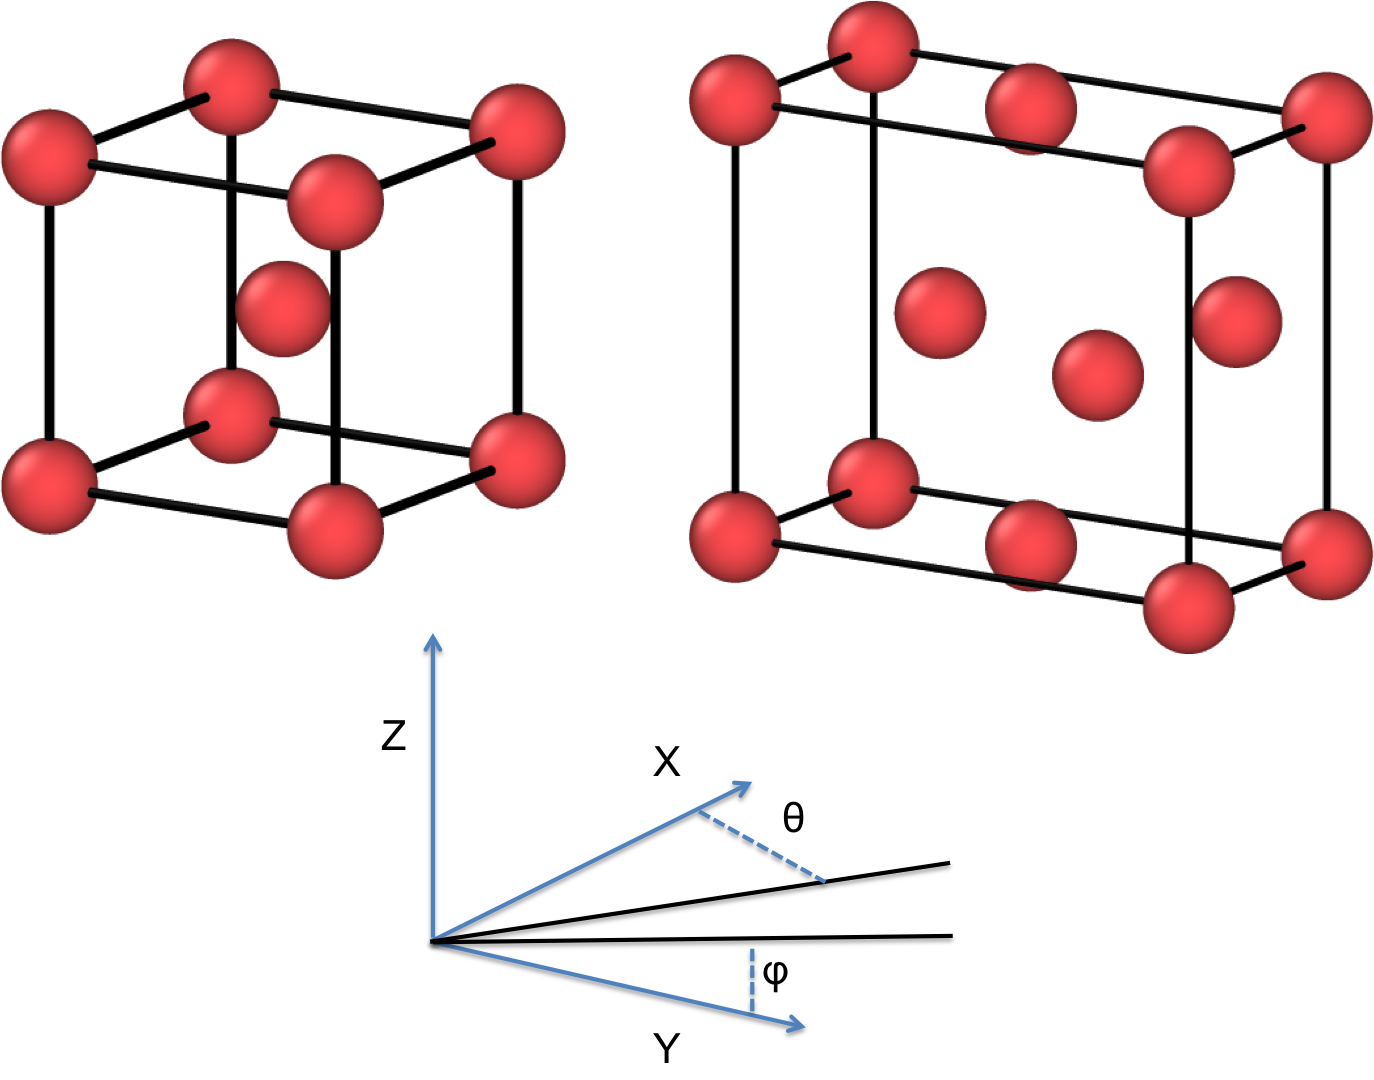
\includegraphics[width=0.5\textwidth]{directionsA.png} 
 \caption{The set of PKA directions are determined by varying the angles $\theta$ and $\phi$. For the $\gamma$ phase (left), $\theta$ is varied from 0\degree to 45\degree and $\phi$ is varied from 0\degree to 35.3\degree. For the $\alpha$ phase (right), $\theta$ is varied from -90\degree to 90\degree and $\phi$ is varied from 0\degree to 90\degree.}
 \label{fig:directions}
\end{figure}

\begin{table}[h]
\caption{The high symmetry directions in $\gamma$ and $\alpha$U and the associated $\theta$ and $\phi$ angles.} \label{tab:dirs}
\begin{center}
\begin{tabular}{|c|c|c|c|}
	\hline
	& Direction & $\theta$ & $\phi$ \\
	 \hline
	 & (1 0 0) & 0 & 0 \\
	$\gamma$U & (1 1 0) & 45 & 0 \\
	& (1 1 1) & 45 & 35.3 \\
	 \hline
	 	 & (1 0 0) & 0 & 0 \\
	$\alpha$U & (0 1 0) & 90 & 0 \\
	& (0 $\bar{1}$ 0) & -90 & 0 \\
	& (0 0 1) & 0 & 90 \\
	 \hline
\end{tabular}
\end{center}
\label{default}
\end{table}


\FloatBarrier

As reviewed by Nordlund, et al.\cite{nordlund2006}, several different definitions of TDE can be introduced. In the previous literature, the primary type of TDE reported is the E$^{\textrm{l}}_{\textrm{d}}$, or the lower bound of the displacement energy, where there exists a non-zero probability of creating a defect \cite{malerba2002}. Typically, the direct experimental measurements of the TDE measure the lowest energy where a defect signal can be detected, for example by changes in resistivity. This is analagous to the E$^{\textrm{l}}_{\textrm{d}}$. For comparison to experiment, adjustments for beam spreading should be included \cite{nordlund2006}. For implementation into the Kinchin-Pease or NRT equations, an average value for the TDE needs to be utilized that is distinct from E$^{\textrm{l}}_{\textrm{d}}$ \cite{nordlund2006,norgett1975}. This average value is obtained from generating probability curves (probability of generating a Frenkel pair as a function of PKA energy) for respective PKA directions. These probability curves can then be averaged over all directions to create an angle-integrated displacement probability curve \cite{nordlund2006}. The energy at which this averaged probability curve crosses the probability 0.5 is determined to be the median TDE (E$^{\textrm{pp}}_{\textrm{d,med}}$), where pp stands for production probability. This value takes into account not only displacement of atoms, but allows for subsequent recombination immediately following the initiation of the cascade (in this work, 14 ps of simulation time following the PKA event). This is the appropriate description of TDE for use in the NRT equation. Only the E$^{\textrm{pp}}_{\textrm{d,med}}$ is calculated in this work.

It should be emphasized that only systems of pure uranium were investigated. Although the UZr MEAM potential and the UMo ADP are capable of describing UZr and UMo alloys, respectively, no such alloy systems were studied in this work. 

\section{Results}
\subsection{$\gamma$U Median Displacement Energy}

In this section, E$^{\textrm{pp}}_{\textrm{d,med}}$ in $\gamma$U is determined at 800 K and 1000 K. For each interatomic potential used (U MEAM \cite{beeler_meam}, UZr MEAM \cite{moore2015} and UMo ADP \cite{smirnovaADP}), the probability of Frenkel pair production as a function of PKA energy is generated for each unique PKA direction. This leads to 55 unique probability curves for each interatomic potential, given that there are 55 unique PKA directions investigated in $\gamma$U. To illustrate the nature of these curves, Fig. \ref{fig:ed_dirall} displays the probability curves for all 55 PKA directions, overlaid with the arithmetic average. Data is generated up to a probability of approximately 0.75 to ensure sampling beyond the median for each PKA direction. The first significant observation is that there is a wide discrepancy between each of the individual directions. Such dramatic variance underlines the importance of gathering a large set of PKA directions to accurately sample the entire phase space of the crystal structure of interest such that true average behavior can be approximated. The second significant observation is that there are non-negligible probabilities of defect production over a wide range of PKA energies, as has been seen before in other materials \cite{beeler2016, nordlund2006, zepeda-ruiz2003, tsuchihira2013}. Finally, the probabilities become non-zero at approximately 20 eV, suggesting that E$^{\textrm{l}}_{\textrm{d}}$ is near 20 eV for this system using this potential, although this value was not strictly determined in this work. Similar variation as a function of PKA direction is observed for the simulations utilizing the UZr MEAM and UMo ADP. For a more precise comparison between directions, three different PKA directions utilizing the U MEAM interatomic potential in $\gamma$U at 800 K are shown in Fig. \ref{fig:ed_dir}. The PKA directions are labeled as \textit{dir2}, \textit{dir24} and \textit{dir28}, which represent the (11.4, 1, 0), (6.2, 3.6, 1) and (4.5, 1.2, 1) directions. The curves shown are fourth order polynomial fits to the data points collected (data points not shown for clarity). The calculated E$^{\textrm{pp}}_{\textrm{d,med}}$ for each individual direction is 36 eV, 58 eV and 101 eV for \textit{dir2}, \textit{dir24} and \textit{dir28}, respectively. This shows a variance in the displacement energy of approximately 70 eV depending on the direction of the PKA. Non-zero probabilities are observed over a range of approximately 100 eV. This is most evident for \textit{dir24}, where probabilities vary from 0.1 at 40 eV, to 0.72 at 140 eV, with the PKA energy of 101 eV yielding a probability of 0.5. Such a large range of non-zero probabilities highlights that the displacement energy at high temperatures is far from the step-function-like description at 0 K \cite{was2007}.
 
 \begin{figure}[h]
 \centering
 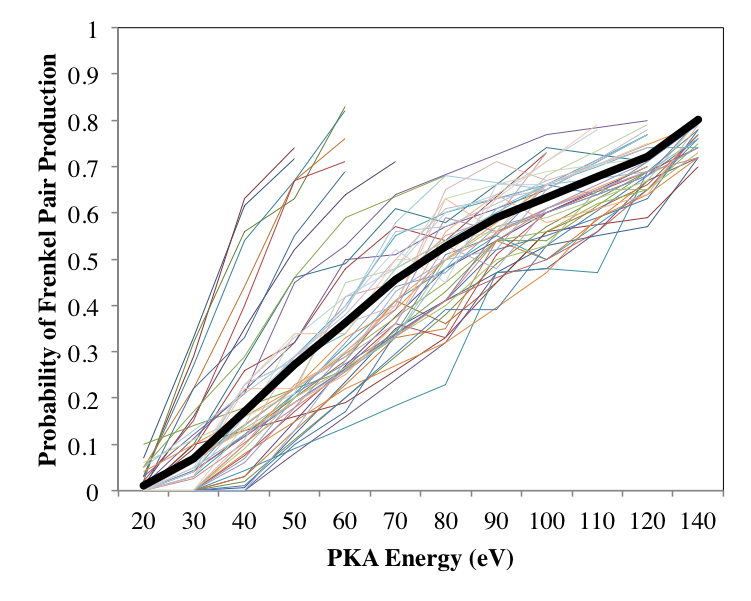
\includegraphics[width=0.8\textwidth]{ed_dir_allC.png} 
 \caption{The Frenkel pair production probability curves in $\gamma$U at 800 K for the U MEAM interatomic potential for all 55 different PKA directions. Average overlaid in black.}
 \label{fig:ed_dirall}
\end{figure}
 
\begin{figure}[h]
 \centering
 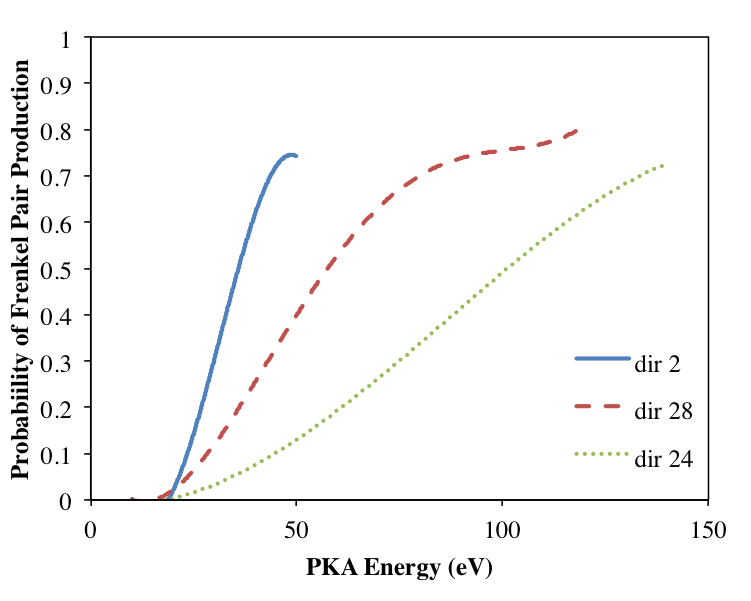
\includegraphics[width=0.8\textwidth]{ed_dirA.png} 
 \caption{The Frenkel pair production probability curves in $\gamma$U at 800 K for the U MEAM interatomic potential in three different PKA directions.}
 \label{fig:ed_dir}
\end{figure}

\FloatBarrier

A full analysis of directional dependence is shown in the contour plot of Figure \ref{fig:800Kcontour}. For each of the three potentials, the displacement energy for a given direction is plotted on a directional field, with the high symmetry directions labelled. Although the magnitude of the threshold displacement energy for each potential is vastly different, as will be discussed below, the directional dependence is very similar. Minima are observed around the (100) direction, while maxima occur at approximately two-thirds along the directional line between the (100) and (110) directions. This maxima is near a (1.75, 1, 0) direction. In the UMo ADP, the maxima is shifted slightly in the z direction. 

\begin{figure}[h]
 \centering
 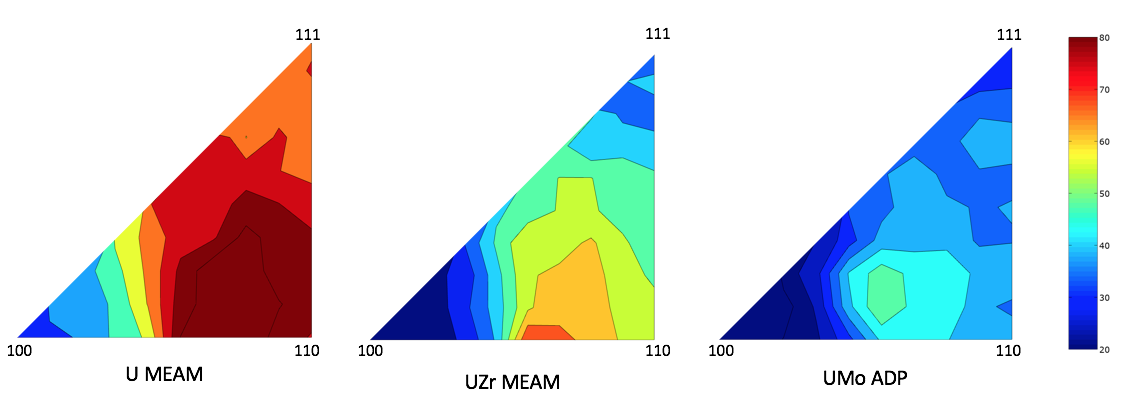
\includegraphics[width=\textwidth]{800K_contour.png} 
 \caption{Contour plots of the displacement energy in $\gamma$U at 800 K for three interatomic potentials. The high symmetry directions are labeled. Units in eV.}
 \label{fig:800Kcontour}
\end{figure}

\FloatBarrier

\subsubsection{Effect of potential on E$^{\textrm{pp}}_{\textrm{d,med}}$ in $\gamma$U}

The probability data from Fig. \ref{fig:ed_dirall} for all PKA directions are arithmetically averaged, creating a single angle-integrated probability curve. This procedure is performed for each of the three interatomic potentials. These three angle-integrated probability curves are displayed in Fig. \ref{fig:gam800} for results at 800 K. In Fig. \ref{fig:gam800} a line is overlaid on the data at a probability of 0.5 over the entire energy spectrum, indicating the median. The major observation from Fig. \ref{fig:gam800} is the significant difference in the results from each of the potentials. There exists a shift right of the curves moving from the UMo ADP to the UZr MEAM to the U MEAM, yielding lowest probabilities for the U MEAM for the same given PKA energy and highest probabilities for the UMo ADP. The value of E$^{\textrm{pp}}_{\textrm{d,med}}$ at 800 K calculated by the U MEAM potential is 74.5 eV; for the UZr MEAM potential, 47 eV; for the UMo ADP potential, 35.6 eV. Given that the number of displacements in the NRT equation \cite{norgett1975} is proportional to E$_{d}^{-1}$, comparing the E$^{\textrm{pp}}_{\textrm{d,med}}$ results for the U MEAM potential and the UMo ADP potential yields a factor of 2 difference in the total number of displacements. This discrepancy is dramatic and points to the importance of selection of interatomic potential, and awareness of the unique behaviors of the potential that is chosen when performing radiation damage simulations. Unfortunately, experimental data does not exist for the displacement energy to determine the E$^{\textrm{pp}}_{\textrm{d,med}}$, and as such the determination of which interatomic potential is displaying accurate behavior is unavailable. 

\begin{figure}[h]
 \centering
 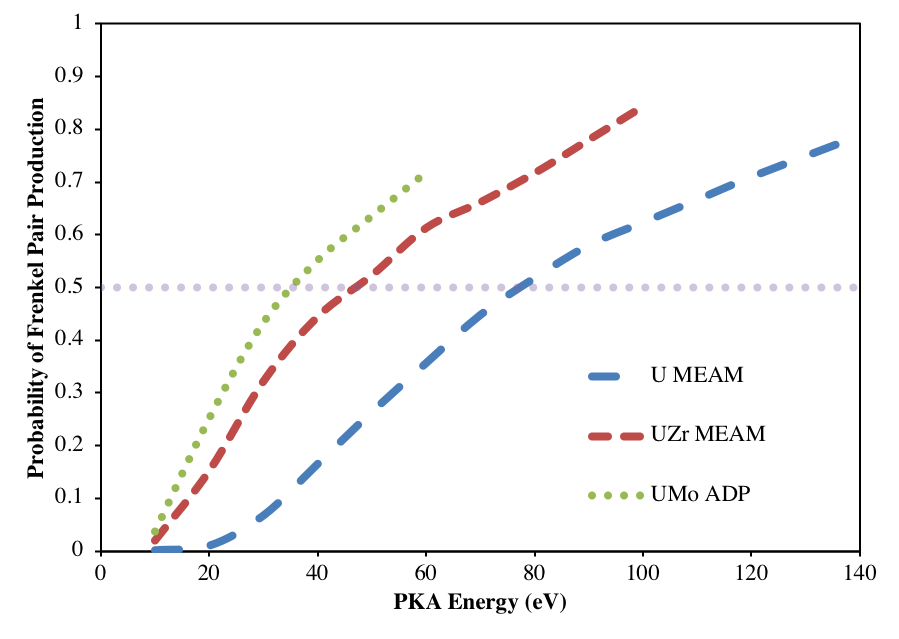
\includegraphics[width=0.8\textwidth]{gam800.png} 
 \caption{The angle-integrated Frenkel pair production probability curves in $\gamma$U at 800 K for three interatomic potentials.}
 \label{fig:gam800}
\end{figure}



\FloatBarrier

In an attempt to understand the nature of the discrepancy between the interatomic potentials, the short range interaction was investigated. A U-U dimer was formed and the energy was analyzed as a function of the dimer distance, shown in Fig. \ref{fig:dimer}. It is observed the the U MEAM and UZr MEAM exhibit similar energy-well minima and similar energy tails as the distance increases (as would be expected, given the similar origins of these two potentials). For the UMo ADP, the energy minimum occurs at a shorter distance and at a higher energy, while the nature of the tail is non-monotonically increasing. At short distances, it is observed that the U MEAM exhibits an increase in energy at the longest r distance, while UMo ADP exhibits an increase in energy at the shortest r distance. It should be explained how the ZBL is implemented within each of these potentials, for clarification and understanding of Fig. \ref{fig:dimer}. For U MEAM and UZr MEAM, the standard ZBL implementation within LAMMPS is employed, which produces ZBL splining cutoffs based on the reference distance and the alpha parameter provided within the potential. This results in ZBL splining cutoffs of 1.27 {\AA} and 2.48 {\AA} for the U MEAM potential and 1.25 {\AA} and 2.43 {\AA} for the UZr MEAM potential. Thus, ZBL splining begins at the longer distance, while below the shorter distance the interaction is purely ZBL. For the UMo ADP, the ZBL is implemented via the hybrid/overlay implementation in LAMMPS, where ZBL cutoffs are manually input. In this work for the UMo ADP, the ZBL splining cutoffs are selected at 1 {\AA} and 2 {\AA}. Thus, for the UMo ADP, ZBL splining begins at 2 {\AA} and below 1 {\AA} the potential is purely ZBL. Based on the nature of the potential wells and the well minimum distance, these are all reasonable choices for ZBL splining criteria. However, there are clear and distinct differences in the low-R energy landscape due to the inherent differences in the ZBL splining. It is most likely not a coincidence that these differences correspond exactly to the differences in displacement energy, whereas U MEAM is the most stiff and displays the highest displacement energy, while UMo ADP is the most soft and displays the lowest displacement energy. Thus, it is suggested that the potential behavior at small distances, governed by the nature of both the energy-well and the ZBL splining, is a primary factor in the observed variation of E$^{\textrm{pp}}_{\textrm{d,med}}$ as a function of interatomic potential. Minor modifications could potentially be made to the ZBL implementation to better fit low-R data in these systems, however no such data exists for $\gamma$U, and as such no modifications were performed for these systems.

\begin{figure}[h]
 \centering
 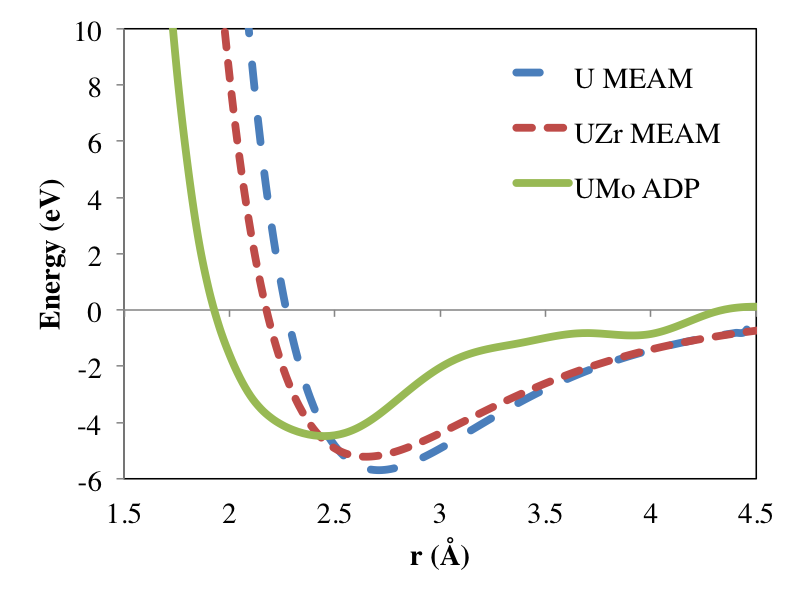
\includegraphics[width=0.6\textwidth]{U_U_dimer.png} 
 \caption{U-U dimer energy versus distance for three different potentials at 0 K.}
 \label{fig:dimer}
\end{figure}


\subsubsection{Effect of temperature on E$^{\textrm{pp}}_{\textrm{d,med}}$ in $\gamma$U}

The results for E$^{\textrm{pp}}_{\textrm{d,med}}$ in $\gamma$U at 800 K and 1000 K are summarized in Table \ref{tab:gam}. Included in Table \ref{tab:gam} in parentheses are a lower and upper bound displacement energy. In order to determine the statistical significance of these results, the standard error of the mean was determined for each data point utilized to construct Fig. \ref{fig:gam800} as well as each data point used to construct the curves for the system at 1000 K. The standard error of the mean for each data point was added to that respective data point in order to create a higher bound probability curve. Likewise, a lower bound probability curve was created by subtracting the standard error of the mean for each respective data point. The upper bound and lower bound E$^{\textrm{pp}}_{\textrm{d,med}}$ is calculated from the point where the upper bound and lower bound probability curves, respectively, cross 0.5 probability. This can provide us with a most probable range (68.2\% confidence interval) for the values of E$^{\textrm{pp}}_{\textrm{d,med}}$. These ranges are provided in Table \ref{tab:gam} in parentheses. 

\begin{table}[h]
\caption{The median displacement energy in $\gamma$U for three different potentials and two temperatures. Energies given in eV. A range incorporating plus/minus one standard error is included in parentheses for each system.} \label{tab:gam}
\begin{center}
\begin{tabular}{|c|c|c|}
	\hline
	& 800 K & 1000 K \\
	 \hline
	 U MEAM & 74.5 (72.9-80.8) & 68.8 (66.4-71.3) \\
	 UZr MEAM & 47.0 (44.5-49.5) & 41.3 (39.8-42.8) \\
	 UMo ADP & 35.6 (33.9-37.4) & 32.8 (31.8-33.7) \\
	 \hline
\end{tabular}
\end{center}
\label{default}
\end{table}

\FloatBarrier

For all three potentials, there is a statistically significant decrease observed in the magnitude of the E$^{\textrm{pp}}_{\textrm{d,med}}$ as temperature increases from 800 K to 1000 K. Previous work performed by the authors have shown the opposite trend in body-centered cubic (bcc) Fe: an increase in the E$^{\textrm{pp}}_{\textrm{d,med}}$ with increasing temperature \cite{beeler2016}. In bcc Fe, this is explained via higher temperatures leading to greater recombination rates, and thus an increase in the difficulty of creating defects that last longer than a few picoseconds after the dissipation of the thermal spike. Previous experimental studies of the E$^{\textrm{l}}_{\textrm{d}}$ in bcc Mo \cite{zag1983} and fcc Cu\cite{yoshida1979} showed a decrease in the displacement energy as a function of temperature, similar to what is shown in Table \ref{tab:gam}. It should be noted that this is a different evaluation of the displacement energy than what is presented in this work or in the work on bcc Fe \cite{beeler2016}- E$^{\textrm{l}}_{\textrm{d}}$ versus E$^{\textrm{pp}}_{\textrm{d,med}}$ - but is included here for completeness. It is unclear if trends present for one interpretation of displacement energy hold for other interpretations. 

Previous studies in bcc Fe \cite{beeler2015, beeler2016} by the authors showed that the trend of the formation energy of a Frenkel pair as a function of applied strain was correlated to the displacement energy as a function of applied strain at a given temperature. Thus, an investigation into Frenkel pair formation energy trends versus temperature for metallic U was undertaken in an attempt to explain the variation in E$^{\textrm{pp}}_{\textrm{d,med}}$ as a function of temperature. Frenkel pair formation energies were determined by equation \ref{eqn:eint}.

\begin{equation}
\label{eqn:eint}
E_{f}^{FP} = E_{int} + E_{vac} - 2*E_{pure}
\end{equation} 

where E$_{int}$ is the energy of a system with an interstitial, E$_{vac}$ is the energy of a system with a vacancy and E$_{pure}$ is the energy of a pure system. E$_{pure}$, E$_{vac}$ and E$_{int}$ were determined by conducting 10 unique simulations for each system. In each simulation, the system is equilibrated for 1 ns at a prescribed temperature, wherein the energy is averaged over the final 500 ps of the simulation. The resultant energy from each of the 10 simulations was averaged to calculate E$_{pure}$, E$_{vac}$ and E$_{int}$. The results for Frenkel pairs, vacancies and interstitials from 800 K to 1200 K in intervals of 100 K are displayed in Table \ref{tab:eform}. Due to statistical fluctuations at high temperatures, there exists an amount of error associated with conducting these simulations. This is the reasoning behind conducting multiple simulations and averaging over the produced set of data. The standard error is calculated as the standard deviation of a set divided by the square root of the sample size. The total error in the formation energy of a Frenkel pair is a sum of the standard error for the 10 simulations for E$_{pure}$, the standard error for the 10 simulations for E$_{vac}$ and the standard error for the 10 simulations for E$_{int}$. The Frenkel pair data in Table \ref{tab:eform} is illustrated in Fig \ref{fig:eform}, on which error bars are included. The average standard error for vacancies and interstitials is approximately 0.13 eV, whereas the average standard error for Frenkel pairs is approximately 0.2 eV. For all defects and potentials, the standard error slightly increases with temperature, due to increased thermal fluctuations. It should be noted that two experimental investigations have been performed to calculate the vacancy formation energy in U, producing results of 1.2$\pm$0.3 \cite{matter1980} and 1.6$\pm$0.2 \cite{lund2013}.

\begin{table}[h]
\caption{The formation energy in $\gamma$U of a Frenkel pair (FP), vacancy (V) and interstitial (I) for three different potentials from 800 K to 1200 K. Energies given in eV.} \label{tab:eform}
\begin{center}
\begin{tabular}{|c|c|c|c|c|c|c|}
	\hline
			& Defect	& 800 K & 900 K & 1000 K & 1100 K & 1200 K\\
	 \hline
			& FP	 & 2.4 & 2.4 & 2.9 & 3.1 & 3.1 \\
	 U MEAM 	& V	& 1.6 & 1.4 & 1.7 & 1.7 & 1.7 \\
	 		& I	& 0.7 & 1.0 & 1.2 & 1.4 & 1.4 \\
	\hline
	 		& FP	& 2.8 & 3.4 & 3.7 & 3.7 & 4.1 \\
	 UZr MEAM & V & 0.8 & 1.7 & 1.5 & 1.4 & 1.9 \\
			& I	& 2.0 & 1.8 & 2.2 & 2.3 & 2.2 \\
	 \hline
	 		& FP	& 3.0 & 2.9 & 3.3 & 3.3 & 3.5 \\
	 UMo ADP & V	& 2.2 & 2.0 & 2.2 & 2.3 & 2.4 \\
	 		& I	& 0.8 & 0.9 & 1.1 & 1.0 & 1.1 \\
	 \hline
\end{tabular}
\end{center}
\label{default}
\end{table}

\begin{figure}[h]
 \centering
 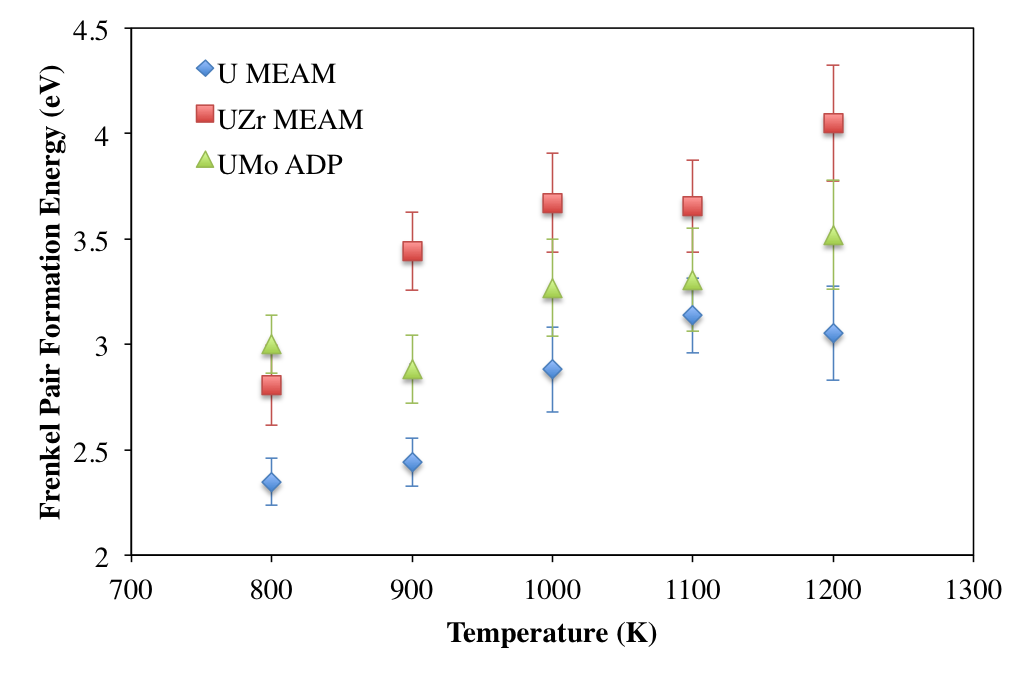
\includegraphics[width=0.8\textwidth]{frenkel_eform.png} 
 \caption{The Frenkel pair formation energy in $\gamma$U for three different potentials from 800 K to 1200 K. Error bars denote plus/minus one standard error.}
 \label{fig:eform}
\end{figure}

\FloatBarrier

For all three potentials, the Frenkel pair formation energy increases from 800 K to 1000 K and generally as a function of temperature. If the Frenkel pair formation energy is positively correlated with the E$^{\textrm{pp}}_{\textrm{d,med}}$, this would suggest an increase in the displacement energy from 800 K to 1000 K, however, the opposite trend is observed in Table \ref{tab:gam}. It is interesting to note the relative magnitudes of the specific point defects for each potential. For the U MEAM and UMo ADP potentials, the interstitial formation energy is lower than the vacancy formation energy. This is in contrast to typical behavior in metals, but consistent with the behavior in $\gamma$U found from DFT \cite{beeler2010}. For the UZr MEAM potential, the formation energy of interstitials is higher than that of vacancies. These relative defect energy magnitudes are consistent for each potential across the entire temperature regime investigated. Since defect energies increase as a function of temperature and defect energies \textit{should} be at least minimally correlated to displacement energy, it can be concluded that there is another factor dominating the temperature trends in the displacement energy other than Frenkel pair formation energy.

\FloatBarrier

Since we know that an increase in temperature generally yields an increase in diffusion, it is worthwhile to investigate the diffusion coefficients and the migration barriers of defect diffusion in $\gamma$U for each of these three potentials over temperatures of interest. Some diffusion studies have been performed utilizing these potentials \cite{smirnovaADP, smirnova2015}, but not for all three potentials, and the results were not fully quantified. Thus a systematic study for all three potentials is warranted.

Utilizing the same simulations that were performed for the calculation of the defect formation energies, the mean square displacement was tracked as a function of time. The total simulation time of 1 ns was deemed to be sufficient as the diffusion coefficient had stabilized and \textit{r}$^{2}$ was linear with time. The calculated diffusion coefficients are shown in Table \ref{tab:diff}, given as a pre-exponential factor (D$_{0}$) and a migration barrier (E$_{m}$). There are no known experimental measurements of the individual interstitial or vacancy diffusion coefficients. Density functional theory studies have been performed to investigate point defects in $\alpha$U \cite{wirth2011}, but no such studies are able to be performed for $\gamma$U due to the mechanical instability of the system at 0 K \cite{beeler2010}.

\begin{table}[h]
\caption{The interstitial (I) and vacancy (V) diffusion coefficient in $\gamma$U for three different potentials over the temperature range of 800 K to 1200 K. Provided as a pre-factor and a migration barrier.} \label{tab:diff}
\begin{center}
\begin{tabular}{|c|c|c|c|}
	\hline
	& Defect & D$_{0}$ (m$^{2}$/s) & E$_{m}$ (eV)\\
	 \hline
	U MEAM & I & 5.999$\times$10$^{-8}$ & 0.228 \\
			& V & 4.767$\times$10$^{-8}$ & 0.305 \\
			\hline
	UZr MEAM & I & 2.345$\times$10$^{-8}$ & 0.086 \\
			& V & 1.179$\times$10$^{-7}$ & 0.341 \\
			\hline
	UMo ADP & I & 3.393$\times$10$^{-8}$ & 0.136 \\
			& V & 1.781$\times$10$^{-7}$ & 0.382 \\
	\hline
\end{tabular}
\end{center}
\label{default}
\end{table}

In order to calculate a self-diffusion coefficient, an average defect formation is utilized (averaged over the temperature range) for both a vacancy and an interstitial. That formation energy is utilized in equation \ref{eqn:selfd}:

\begin{equation}
\label{eqn:selfd}
D_{self} = D^{int}_{0} \times exp(-E_{int}/kT) + D^{vac}_{0} \times exp(-E_{vac}/kT)
\end{equation} 

where D$^{int}_{0}$ and D$^{vac}_{0}$ are the pre-factors from Table \ref{tab:diff} and E$_{int}$ and E$_{vac}$ are the averaged formation energies from Table \ref{tab:eform}. The calculated self-diffusion coefficients are displayed in Fig \ref{fig:gamUdiff}. An experimental result is provided as a comparison \cite{adda1959}. Very little other experimental data is available for comparison. Further experimental studies are warranted, as a single experimental reference is insufficient to provide full confidence in the true values of self-diffusion in $\gamma$U. The UMo ADP most closely matches experiment, as has been shown in \cite{smirnovaADP}. The U MEAM underestimates the self-diffusion coefficient, while the UZr MEAM overestimates the self-diffusion coefficient. It is interesting that although the diffusion of interstitials is faster than vacancies, as expected, the difference is less than one order of magnitude for all potentials investigated. Thus, self-diffusion will occur via both vacancy and interstitial mechanisms, as has been previously suggested \cite{fedorov1978, smirnov1992}. As expected, diffusion coefficients increase as temperature increases for all potentials. An increase in diffusion should result in an increase in recombination making it more difficult to create permanent defects and thus yielding an increase in displacement energy, as was observed in bcc Fe \cite{beeler2016}. However, the opposite trend seems to be in place for $\gamma$U. It can be concluded that variations in diffusion behavior as a function of temperature are not responsible for the decrease in displacement energy as a function of temperature.

\begin{figure}[h]
 \centering
 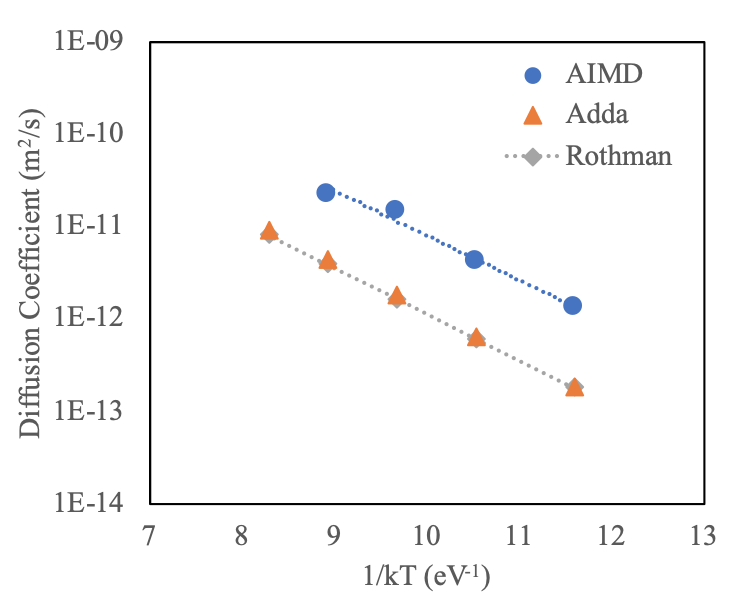
\includegraphics[width=0.8\textwidth]{self_diff.png} 
 \caption{The self-diffusion coefficient in $\gamma$U for three different potentials from 800 K to 1200 K. An experimental study is included for comparison \cite{adda1959}.}
 \label{fig:gamUdiff}
\end{figure}

\FloatBarrier

In a further attempt to understand this variation of displacement energy as a function of temperature, the calculation of elastic constants from 800 K to 1200 K was performed. Typically, elastic constants soften as a function of temperature \cite{varshni1970}. Softening of elastic constants \textit{should} result in a lower displacement energy, as the lattice is more easily deformed. Elastic constants were calculated by performing displacements of the system and using the resultant changes in stress to compute the elastic stiffness tensor, as provided by the LAMMPS distribution. There exists a large amount of thermal fluctuation in these systems, leading to a large amount of variation in the elastic constant calculations. In spite of the thermal noise, clear trends can be obtained for the elastic constants as a function of temperature, given that sufficiently robust sampling is performed. In order to achieve some statistical certainty for each simulation of elastic constants, 100 samples are taken, with a sampling interval of 10 timesteps, as defined within the LAMMPS elastic constant scripts. The systems are equilibrated for 100 ps, a deformation is performed, and the systems are re-equilibrated for 50 ps in order to obtain the subsequent changes in the stress tensor. This simulation produces the nine elastic constants, or the complete stress tensor. Given that the bcc system is cubic, C$_{11}$, C$_{22}$ and C$_{33}$ are identical and are thus averaged to obtain C$_{11}$. Similar averaging was performed to obtain C$_{12}$ and C$_{44}$. Six unique calculations were performed for each given temperature and interatomic potential in order to obtain averages of the elastic constants. This leads to the standard deviation across all systems of approximately plus or minus 5 GPa for a given elastic constant at a given temperature for a given potential. This is an acceptable amount of uncertainty to obtain quantitative values of the elastic constants and their respective trends as a function of temperature. The results of these simulations are displayed in Fig. \ref{fig:elastic}. The data points are overlaid with a linear fit to the data points to emphasize the trends in behavior versus temperature. There is some scatter in the data due to the fact that these are high temperature systems, but clear trends are observed. 

For all three potentials, there is a general softening of elastic constants as a function of temperature. Each potential shows a varying degree of softening with temperature, and the magnitude of the various elastic constants is not the same across all potentials. The most notable difference is the very low value of C$_{44}$ for the U MEAM potential. The bulk modulus is calculated as B=($C_{11}$+2$\times$C$_{12}$)/3. The bulk modulus as a function of temperature is shown in Fig. \ref{fig:bulk}. The experimentally observed bulk modulus for $\gamma$U is 113 GPa\cite{yoo1998}, which is higher than the results for any of the potentials. It is observed that the UZr MEAM potential provides the most stiff elastic response, while U MEAM is the softest. This corresponds reasonably well to the relative magnitudes of the Frenkel pair formation energies for each of the potentials, with the UZr MEAM exhibiting the highest Frenkel pair formation energy and U MEAM the lowest. It is also observed that the UMo ADP exhibits the least amount of softening as a function of temperature, while the UZr MEAM expresses the greatest amount of softening with increasing temperature. This qualitatively correlates to relative softening of the E$^{\textrm{pp}}_{\textrm{d,med}}$ with increasing temperature, as UZr MEAM shows the largest percentage decrease from 800 K to 1000 K and UMo ADP shows the smallest percentage decrease. Thus, it is plausible that the softening of elastic constants contributes to the reduction in the TDE as temperature increases, as a softer lattice would be more easily deformed. 


\begin{figure}[h]
 \centering
 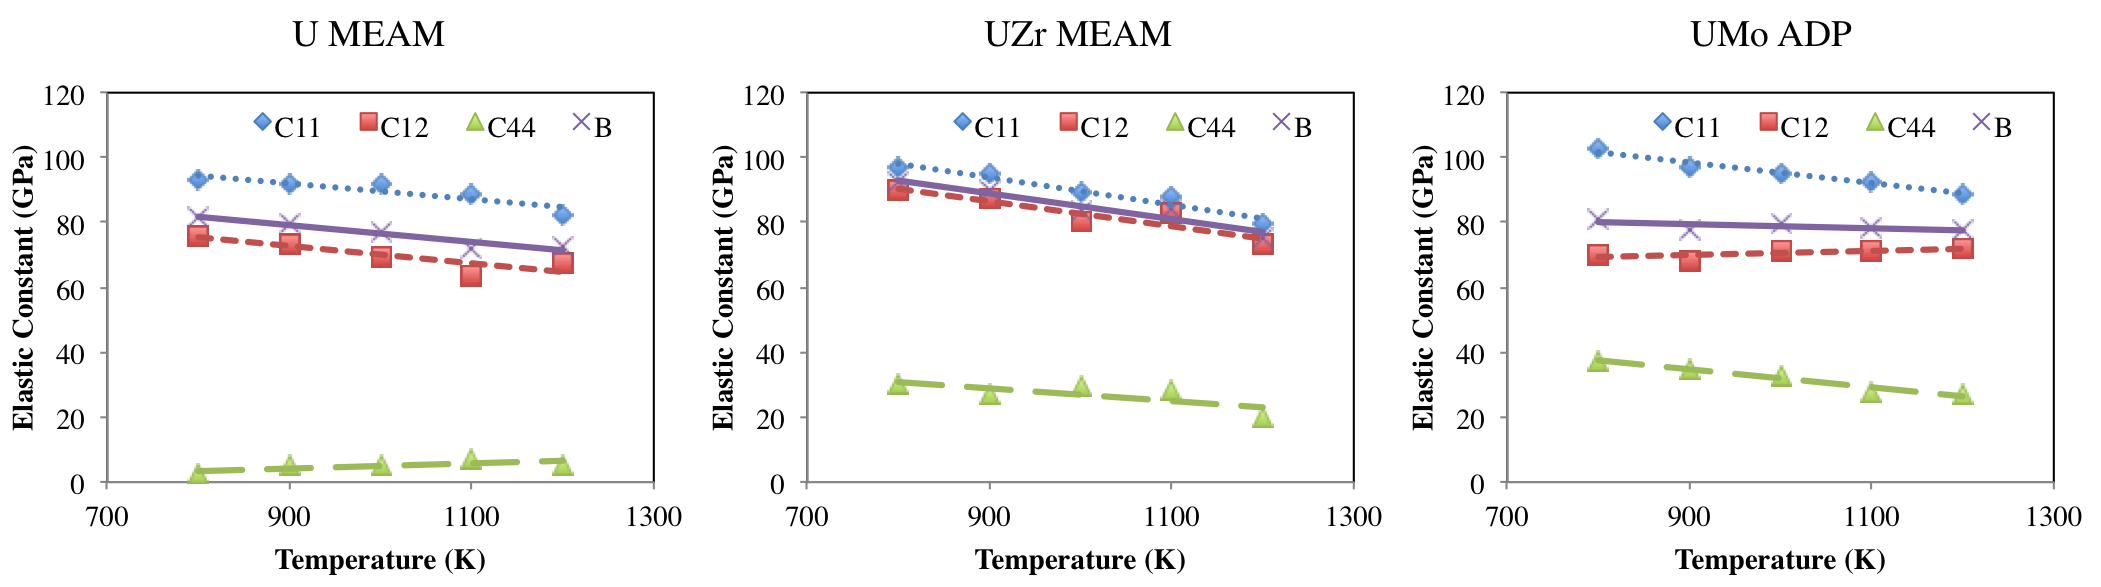
\includegraphics[width=\textwidth]{elastic_vs_T.png} 
 \caption{The elastic constants as a function of temperature in $\gamma$U for three different potentials from 800 K to 1200 K.}
 \label{fig:elastic}
\end{figure}

\begin{figure}[h]
 \centering
 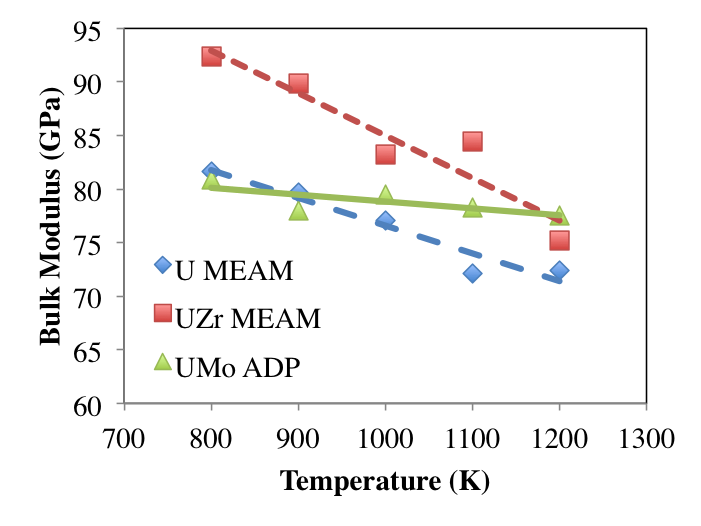
\includegraphics[width=0.6\textwidth]{bulk_vs_Tb.png} 
 \caption{The bulk modulus as a function of temperature in $\gamma$U for three different potentials from 800 K to 1200 K.}
 \label{fig:bulk}
\end{figure}

\FloatBarrier

\subsection{$\alpha$U Median Displacement Energy}

In this section, E$^{\textrm{pp}}_{\textrm{d,med}}$ in $\alpha$ U is determined at 600 K and 800 K. This work utilized the UMo ADP \cite{smirnovaADP}. The probability of Frenkel pair production as a function of PKA energy is generated for each unique PKA direction. This leads to 118 unique probability curves for each interatomic potential. To illustrate the nature of these curves, Fig. \ref{fig:ed_diralpha} displays the probability curves for all 118 PKA directions, overlaid with the arithmetic average. Data is generated up to a probability of approximately 0.75 to ensure sampling beyond the median for each PKA direction. Similar to $\gamma$U in Fig. \ref{fig:ed_dir}, there exists a strong dependence on the direction of the PKA. Whereas the system of $\gamma$U shown in Fig. \ref{fig:ed_dir} shows a variance in the displacement energy across PKA directions of approximately 70 eV, in the $\alpha$U system at 600 K there is an observed variance across directions of over 100 eV. Given that $\alpha$U is a more complex crystal system, high symmetry and low symmetry directions possess incredibly different characteristics and this is reflected in the stark variance across crystallographic directions for the PKA. The authors would again like to emphasize the importance of gathering a large set of PKA directions to accurately sample the entire phase space of the crystal structure of interest such that true average behavior can be approximated. 

\begin{figure}[h]
 \centering
 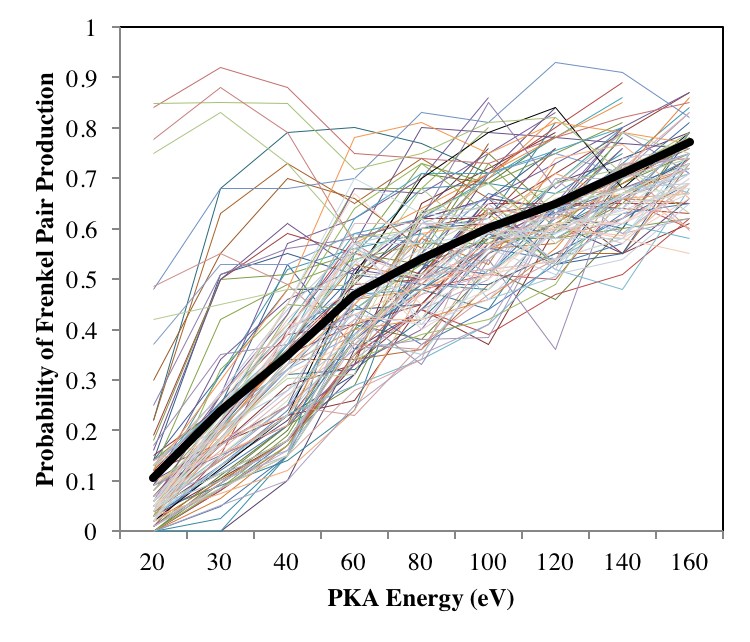
\includegraphics[width=0.8\textwidth]{ed_dir_allD_alpha.png} 
 \caption{The Frenkel pair production probability curves in $\alpha$U at 600 K for the UMo ADP in all 118 different PKA directions. Average overlaid in black.}
 \label{fig:ed_diralpha}
\end{figure}

\FloatBarrier

A full analysis of directional dependence is shown in the contour plot of Figure \ref{fig:600Kcontour}. The displacement energy for a given direction is plotted on a directional field, with the primary directions labelled. The resultant contour field is very complex, as would be expected from a very complex crystal structure. The largest area of minima exists along the (100) to (0$\bar{1}$0) line, at approximately a (1, -2, 0) direction. This is essentially the diagonal of the base of the $\alpha$U structure, and as such could be considered a relatively high symmetry direction. Several areas of local maxima exist, three of which occur near the (0, 1, 2.5), (2, 0, 1) and (0, -3, 1) directions. 

\begin{figure}[h]
 \centering
 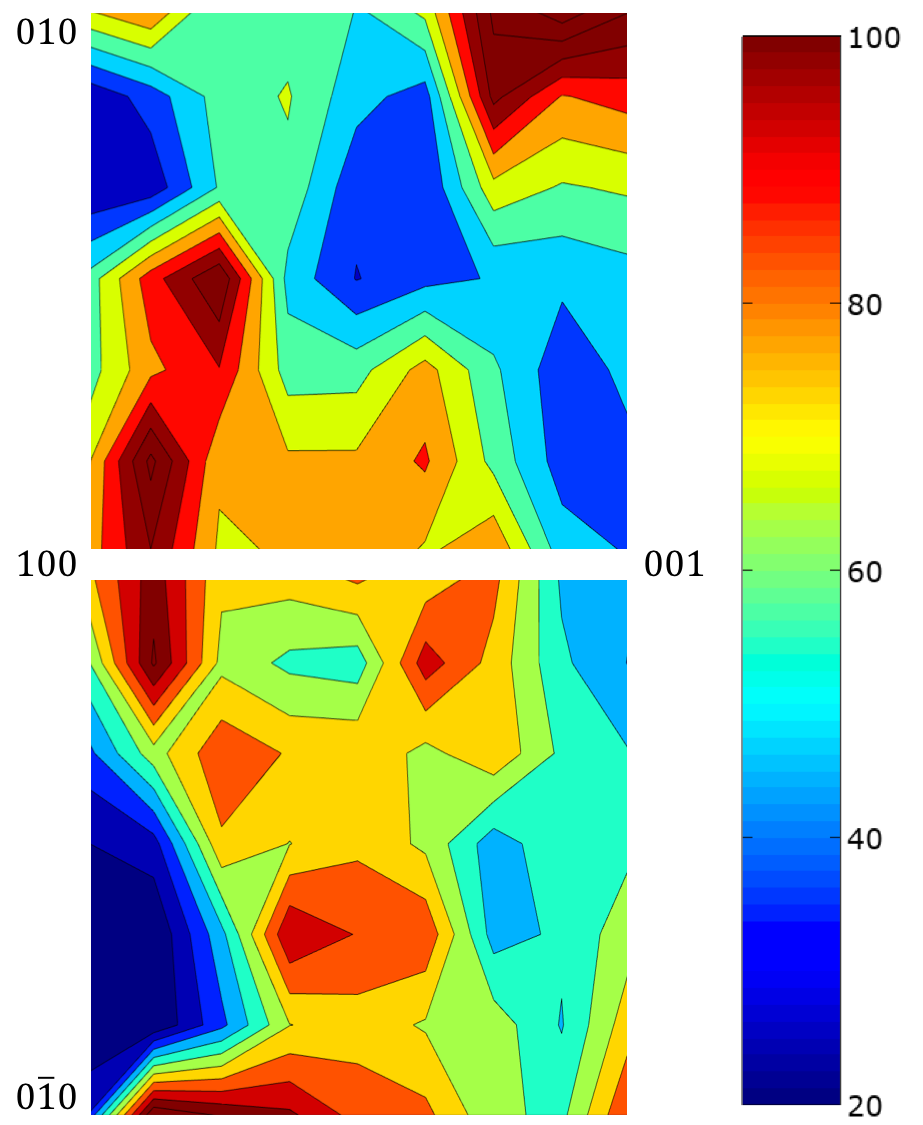
\includegraphics[width=0.6\textwidth]{600K_contour.png} 
 \caption{Contour plot of the displacement energy in $\alpha$U at 600 K for the UMo ADP interatomic potential. The primary directions are labeled. Units in eV.}
 \label{fig:600Kcontour}
\end{figure}

\FloatBarrier

The probability curves from Figure \ref{fig:ed_diralpha} for all PKA directions are arithmetically averaged, creating a single angle-integrated probability curve. The angle-integrated probability curves at 600 K and 800 K for the UMo ADP are displayed in Fig. \ref{fig:alpha}. A line is overlaid on the data in Fig. \ref{fig:alpha} at a probability of 0.5 over the entire energy spectrum, indicating the median. The major observation from Fig. \ref{fig:alpha} is the minimal difference in the results from 600 K to 800 K. The value of E$^{\textrm{pp}}_{\textrm{d,med}}$ at 600 K is 66.2 eV and the value at 800 K is 62.8 eV. This slight decrease is in accordance with the previous trends in $\gamma$U, however this trend is not quite statistically significant. An upper bound and lower bound of the E$^{\textrm{pp}}_{\textrm{d,med}}$ were calculated for $\alpha$U, similar to the calculations above for $\gamma$U. The most probable range for E$^{\textrm{pp}}_{\textrm{d,med}}$ at 600 K is 63.6-68.8 eV, while at 800 K the most probable range is 60.8-64.9 eV. These results suggest that in $\alpha$U, unlike $\gamma$U, any variance in defect energetics, diffusion, or elastic constants between 600 K and 800 K yields very minor discernible difference in the TDE.

\begin{figure}[h]
 \centering
 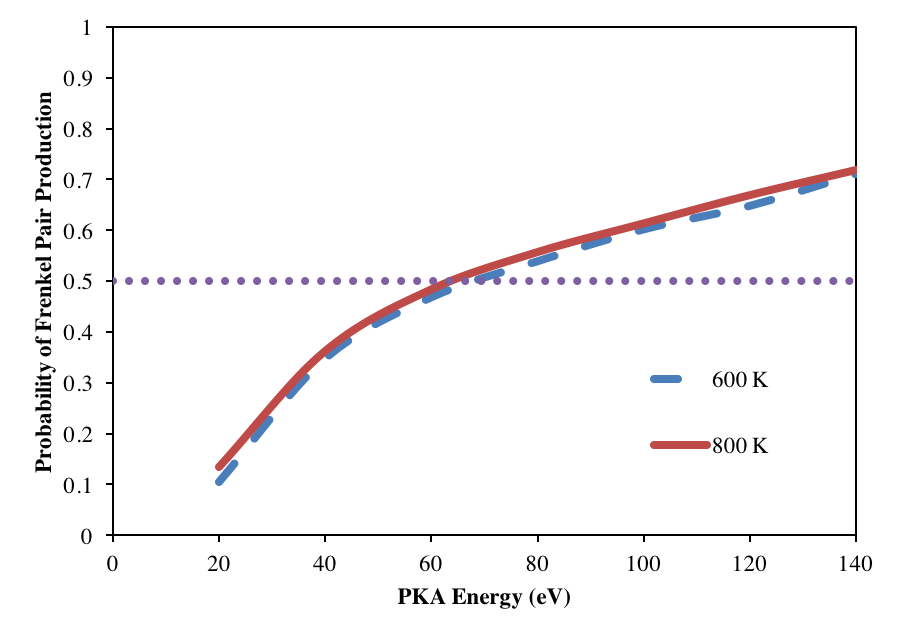
\includegraphics[width=0.8\textwidth]{alpha.png} 	
 \caption{The angle-integrated Frenkel pair production probability curves at 600K and 800 K for $\alpha$U using the UMo ADP.}
 \label{fig:alpha}
\end{figure}

\FloatBarrier

To investigate defect behavior in $\alpha$U, a set of simulations was conducted at 600 K and 800 K to ascertain the defect formation energies in $\alpha$U at each of these respective temperatures. Utilizing equation \ref{eqn:eint}, E$_{pure}$, E$_{vac}$ and E$_{int}$ were determined by conducting ten unique simulations for each system. In each simulation, the system is equilibrated for 1 ns at a prescribed temperature, wherein the energy is averaged over the final 500 ps of the simulation. The resultant energy from each of the ten simulations was averaged to calculate E$_{pure}$, E$_{vac}$ and E$_{int}$. The defect formation energies are presented in Table \ref{tab:alphadef}. The diffusion coefficients were also determined at 600 K and 800 K. Utilizing the same simulations that were conducted to determine defect formation energies, the mean square displacement was tracked as a function of time. The total simulation time of 1 ns was deemed to be sufficient as the diffusion coefficient had stabilized and \textit{r}$^{2}$ was linear with time. The calculated diffusion coefficients allowed for the determination of a migration barrier (E$_{m}$) and pre-factor (D$_{0}$), displayed in Table \ref{tab:alphadiff}.

\begin{table}[h]
\caption{The interstitial, vacancy and Frenkel pair formation energies in $\alpha$U for the UMo ADP at 600 K and 800 K. Units in eV.} \label{tab:alphadef}
\begin{center}
\begin{tabular}{|c|c|c|}
	\hline
	Defect & 600 K & 800 K\\
	 \hline
	Frenkel Pair	& 4.1 & 4.8 \\
	Vacancy		& 1.5 & 1.6 \\
	Interstitial		& 2.6 & 3.2 \\
	\hline
\end{tabular}
\end{center}
\label{default}
\end{table}

\begin{table}[h]
\caption{The interstitial (I) and vacancy (V) diffusion coefficient in $\alpha$U for the UMo ADP over the temperature range of 600 K to 800 K. Provided as a pre-factor and a migration barrier.} \label{tab:alphadiff}
\begin{center}
\begin{tabular}{|c|c|c|}
	\hline
	Defect & D$_{0}$ (m$^{2}$/s) & E$_{m}$ (eV)\\
	 \hline
	 I & 2.172$\times$10$^{-7}$ & 0.35 \\
	 V & 1.148$\times$10$^{-7}$ & 0.34 \\
	\hline
\end{tabular}
\end{center}
\label{default}
\end{table}

\FloatBarrier

Compared to density functional theory values from Wirth \cite{wirth2011}, the vacancy formation energy is quite accurate, while the interstitial energy is substantially underestimated (DFT values of 1.69 eV and 4.42 eV for vacancy and interstitial formation energy, respectively), but it should be noted that these values are for systems are 0 K. The vacancy migration energy compares excellently (DFT value of 0.34 eV), but the interstitial migration energy is overestimated (DFT value of 0.19 eV). In $\alpha$U, this leads to an activation energy for vacancies that is much lower than that of interstitials, suggesting self-diffusion occurs via a vacancy mechanism, as is typical in metals (and in opposition to the behavior in $\gamma$U). 

\subsection{Comparison of $\alpha$U and $\gamma$U displacement energies}

Finally, the results for displacement energy in $\alpha$U need to be compared to the results from $\gamma$U. Utilizing the same potential to compare two phases is the most direct way to approach this comparison, thus the results for only the UMo ADP will be discussed. At 800 K, $\alpha$U exhibits a TDE of 62.8 eV and $\gamma$U exhibits a TDE of 35.6 eV. Thus, it is much more probable for a PKA of a given energy to generate a defect in $\gamma$U than in $\alpha$U. This corresponds to the difference in Frenkel pair formation energy between $\alpha$U and $\gamma$U for the UMo ADP, as the Frenkel pair formation energy is 4.8 eV for $\alpha$U and 3.0 eV for $\gamma$U. The self-diffusion coefficient at 800 K (taken from defect energies and diffusion coefficients and using equation \ref{eqn:selfd}) for $\gamma$U is five orders of magnitude higher than that of $\alpha$U, largely due to the dramatically lower interstitial formation energy of $\gamma$U. Thus, the results from the defect analyses are in concordance with the displacement energy simulation results, with the conclusion that a PKA of a given energy is more likely to produce a defect in $\gamma$U than in $\alpha$U. 

\FloatBarrier

\section{Conclusions}

In this study, molecular dynamics simulations were performed to calculate the displacement energy in $\alpha$ and $\gamma$U at 600 K, 800 K and 1000 K utilizing three unique interatomic potentials. The probability of Frenkel pair production was determined as a function of PKA direction and temperature. Probability curves are averaged to determine an effective value of the TDE (E$^{\textrm{pp}}_{\textrm{d,med}}$), above which a Frenkel pair is more than 50$\%$ likely to form. The value of E$^{\textrm{pp}}_{\textrm{d,med}}$ for $\gamma$U strongly depends on the interatomic potential utilized, as values range from 36 eV to 75 eV at 800 K. This is explained via the differences in the short range interactions for each of the potentials. It is found that for $\gamma$U, displacement energy decreases with increasing temperature. Defect energetics, diffusion coefficients and elastic constants were calculated to investigate this phenomenon. It is found that the negative correlation of the E$^{\textrm{pp}}_{\textrm{d,med}}$ with temperature is possibly due to the softening of elastic constants with increasing temperature. Finally, the TDE in $\alpha$U is found to be higher than in $\gamma$U. Thus, one would expect it to be more difficult to generate a defect in $\alpha$U than in $\gamma$U.

\section{Acknowledgement}
This work was supported by the U.S. High Performance Research Reactor (USHPRR) Fuel Qualification (FQ) Program. This manuscript has been authored by Battelle Energy Alliance, LLC under Contract No. DEAC07-05ID14517 with the U.S. Department of Energy. The United States Government retains, and the publisher, by accepting the article for publication acknowledges that the United States Government retains, a nonexclusive, paid-up, irrevocable, world-wide license to publish or reproduce the published form of this manuscript, or allow others to do so, for United States Government purposes. This research made use of the resources of the High Performance Computing Center at Idaho National Laboratory, which is supported by the Office of Nuclear Energy of the U.S. Department of Energy and the Nuclear Science User Facilities under Contract No. DE-AC07-05ID14517.

\bibliography{MARMOTbib}

\end{document} 
